
\documentclass[12pt,a4paper,USenglish]{article}
\usepackage{ae}
\usepackage{babel}
\usepackage[utf8x]{inputenc}
\usepackage{ucs}
\usepackage[T1]{fontenc}
\usepackage{t1enc}
\usepackage{type1cm}
\usepackage[pdftex,pagebackref=true]{hyperref}
\hypersetup{
    colorlinks,
    citecolor=black,
    filecolor=black,
    linkcolor=black,
    urlcolor=black,
    unicode=true,
    bookmarksopen=true,     % Gliederung öffnen im AR
    bookmarksnumbered=true, % Kapitel-Nummerierung im Inhaltsverzeichniss anzeigen
    bookmarksopenlevel=1,   % Tiefe der geöffneten Gliederung für den AR
    pdfstartview=FitV,       % Fit, FitH=breite, FitV=hoehe, FitBH
    pdfpagemode=UseOutlines, % FullScreen, UseNone, UseOutlines, UseThumbs 
}
\usepackage{graphicx}
\IfFileExists{url.sty}{\usepackage{url}}
                      {\newcommand{\url}{\texttt}}

%\makeatletter
%\makeatother

\sloppy

\begin{document}

\title{CoopSim - \\A Computer Simulation of the Evolution of Cooperation\\User's Manual}
\author{Eckhart Arnold}
\date{September, 6th 2015}

\maketitle

\tableofcontents{}


\section{Introduction}

\emph{CoopSim} is a computer simulation of the reiterated prisoner's
dilemma. The reiterated prisoner's dilemma is a model for many (but
not for all) cooperation dilemmas discussed in social sciences.
It is also useful as a model for the evolution of altruistic behaviour
in biology. The computer program \emph{CoopSim} has been written for
use in an undergraduate course on the ``Evolution of Cooperation''.
Its purpose is mainly educational.

The reiterated prisoner's dilemma and its simulation on the computer
is discussed in a very understandable form in the book ``The Evolution
of Cooperation'' by Robert Axelrod. Therefore, it will not be explained
here any more (see section ``Further Reading'' for some recommendable
books on the topic). A basic knowledge of what the \emph{prisoner's dilemma}
is and what it has got to do with altruism and cooperation is presupposed
in the following. The program \emph{CoopSim} is largely based on the
description of Axelrod's book. However, the whole program has been
written from scratch without taking recourse to Axelrod's original
Fortran program. I did so, because I wanted the program code to be
readable enough so that students with some programming knowledge might
be encouraged to extend the program and to implement strategies of
their own. Also, I wanted the simulation to have a nice user interface
so that I could do ``life'' simulations under different boundary
conditions in class.

\section{Aknowledgements}

\emph{CoopSim} is based on the description of a computer tournament
in Robert Axelrod's book ``The Evolution of Cooperation''. The
nomenclature (``computer tournament'', ``ecological simulation'') has
been taken from this book. Some of the strategies built into
\emph{CoopSim} are (sometimes only loosely) based on strategies with
the same name described in Axelrods book.

I would also like to thank the following people for contributing
strategies of their own: Alex Mainzer, Björn van den Bruck, 
Christian Erlen, Stefan Pennartz, Sven Sommer, Paul Boehm.

Finally, I would like to thank the initiators, makers and contributers
to the \emph{Python} programming language (www.python.org
\url{www.python.org}) and the \emph{wxWidgets} GUI-Toolkit
(www.wxwidgets.org \url{www.wxwidgets.org}; www.wxpython.org
\url{www.wxpython.org}). \emph{Python} and \emph{wxWidgets} are open
source software packages without which the making of \emph{CoopSim}
would not have been possible in this form.

\section{License}

The MIT License (MIT)

Copyright (c) 2004 Eckhart Arnold (eckhart\_arnold@yahoo.de, www.eckhartarnold.de)

Permission is hereby granted, free of charge, to any person obtaining a copy
of this software and associated documentation files (the "Software"), to deal
in the Software without restriction, including without limitation the rights
to use, copy, modify, merge, publish, distribute, sublicense, and/or sell
copies of the Software, and to permit persons to whom the Software is
furnished to do so, subject to the following conditions:

The above copyright notice and this permission notice shall be included in
all copies or substantial portions of the Software.

THE SOFTWARE IS PROVIDED "AS IS", WITHOUT WARRANTY OF ANY KIND, EXPRESS OR
IMPLIED, INCLUDING BUT NOT LIMITED TO THE WARRANTIES OF MERCHANTABILITY,
FITNESS FOR A PARTICULAR PURPOSE AND NONINFRINGEMENT. IN NO EVENT SHALL THE
AUTHORS OR COPYRIGHT HOLDERS BE LIABLE FOR ANY CLAIM, DAMAGES OR OTHER
LIABILITY, WHETHER IN AN ACTION OF CONTRACT, TORT OR OTHERWISE, ARISING FROM,
OUT OF OR IN CONNECTION WITH THE SOFTWARE OR THE USE OR OTHER DEALINGS IN
THE SOFTWARE.

\section{Installation}

\subsection{System Requirements}

\noindent \textbf{Hardware Requirements:}

\begin{itemize}
\item AMD Athlon or Pentium III System, 1 Ghz or above (otherwise
\emph{CoopSim} might run pretty slow)
\item 128 MB or more of memory

\end{itemize}

\noindent \textbf{Software Requirements:}

\begin{itemize}
\item Linux or Windows 98/XP Operating System
\item Python 2.3 or above (\url{www.python.org})
\item wxPython 2.4 or above (\url{www.wxpython.org})
\end{itemize}

\subsection{Installing CoopSim}

To install and successfully run {\em CoopSim} you need to have Python
version 2.3 or above and wxPython version 2.4 or above installed on
your System. You can download the installation packages from the websites
mentioned above. \emph{CoopSim} runs under Windows, Linux and potentially 
under MacOS as well, but it has only been tested under Windows and Linux.
In order to install \emph{CoopSim} you only need to unpack the zip archive
``CoopSim.zip'' anywhere on your hard disk.


\subsection{Running ''CoopSim''}

To run \emph{CoopSim}, you have to start the executable python file
``CoopSim.py'' in the main installation directory either by double
clicking or by changing to the CoopSim directory and entering ``python
CoopSim.py'' at the command line.


\section{First Steps - A guided tour through \emph{CoopSim}}


\subsection{Starting a predefined simulation}

After successfully starting CoopSim you should see an application
Window like this:

\begin{center}
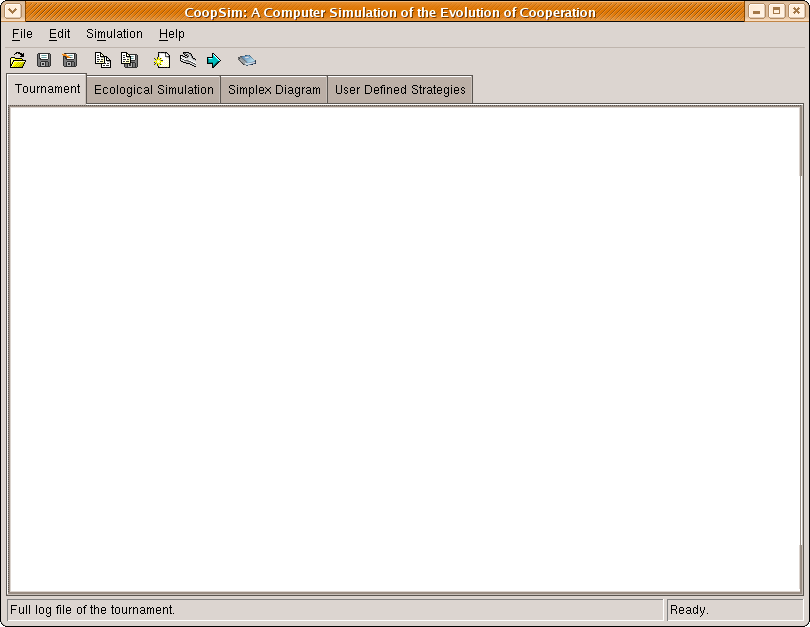
\includegraphics[width=8cm,keepaspectratio]{big_images/app_start.png}
\end{center}

In the beginning the screen is empty, of course. You will notice four notebook
pages named: \emph{Tournament}, \emph{Ecological Simulation}, \emph{Simplex
  Diagram} and \emph{User Defined Strategies}. The purpose of these pages will
be explained later. First, we will just start the simulation \emph{Simple
  Example}. This simulation is preselected when the program starts up (you can
see which simulation is active and which simulations are available in the
\emph{Simulation} menu), so it is just enough to click the \emph{Continue
  Simulation} button to start the simulation. This is the button with the
blue arrow pointing to the right. It is the second button from the left
in the button row under the menu. After a short time of calculating the result
of the tournament should appear on the \emph{Tournament} page:

\begin{center}
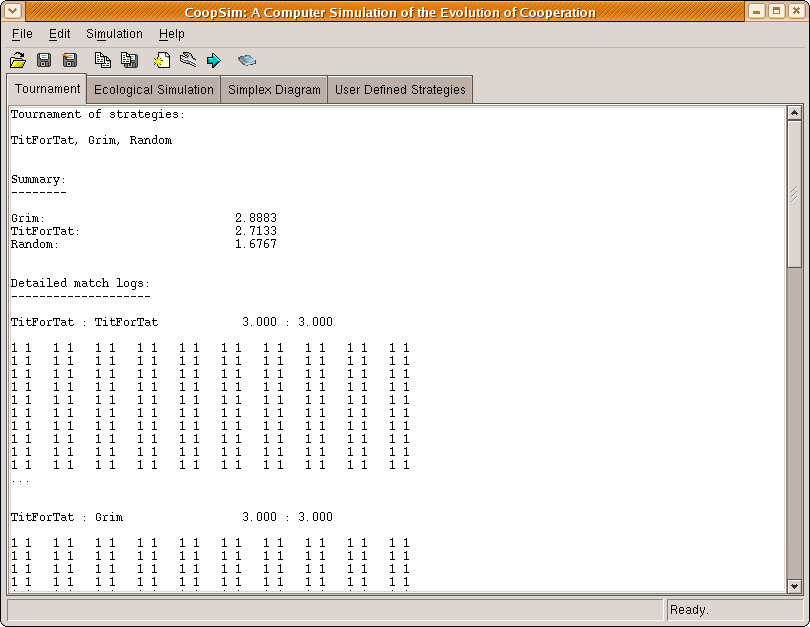
\includegraphics[width=8cm,keepaspectratio]{big_images/tournament_page.png}
\end{center}

The tournament page displays the following information:

\begin{enumerate}
\item The strategies that took part in the tournament.
\item Then ranking of the strategies.
\item The outcome of each single match of a pair of strategies as well as
the first and last 50 moves of the players, where {\bf 0} indicates a defection
and a {\bf 1} a cooperative move.
\item The ranking of the strategies in the ecological simulation after a
certain number of generations.
\end{enumerate}

You can scroll the contents of the text window using the slider on the
right side in order to see all the information. As you can see from the
tournament log, the simulation \emph{Simple Example} is a tournament
of three strategies only: GRIM, TITFORTAT and RANDOM. Among these
three strategies GRIM emerges as the clear winner.

Now, let us have a look at the other notebook pages. Select the page
\emph{Ecological Simulation} in order to view the graph of the ecological
simulation. The graph shows the population dynamics of the strategies
in the tournament, assuming that the fitness of a strategy is
determined by its score in the tournament. It should look like this:

\begin{center}
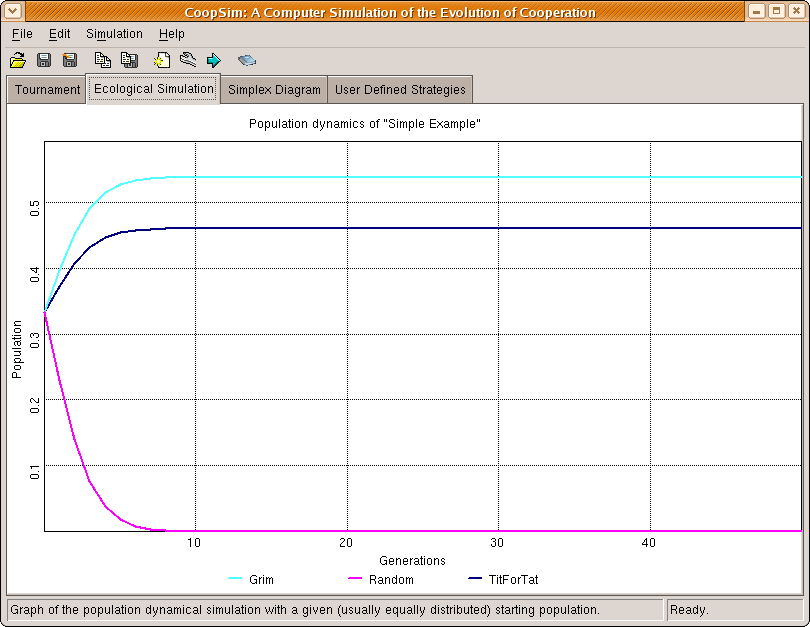
\includegraphics[width=8cm,keepaspectratio]{big_images/eco_page.png}
\end{center}

If you wonder how the development is going to continue after the 50th
generation (you probably don't when the graph is as simple as in this case, but
sometimes it takes more generations until a clear result crystalizes out), you
can click on the blue arrow button again to let the simulation continue. You
can do this as often as you like. (To go back to the first 50 generations,
just restart the simulation from the {\em Simulation} menu.)

Now suppose you would like to save the graph (maybe, because you are
just about to write a paper on cooperation in the reiterated prisoner's
dilemma, for which some graphical illustrations might be useful).
You can do so by selecting \emph{Save Page As} from the \emph{Edit}
menu or by clicking the \emph{Save Page} button in the toolbar (somewhere
in the middle, not to be confused with the \emph{Save} button which
saves the whole setup of simulations!). A dialog box will appear where
you can the select a directory and enter a filename for the graph:

\begin{center}
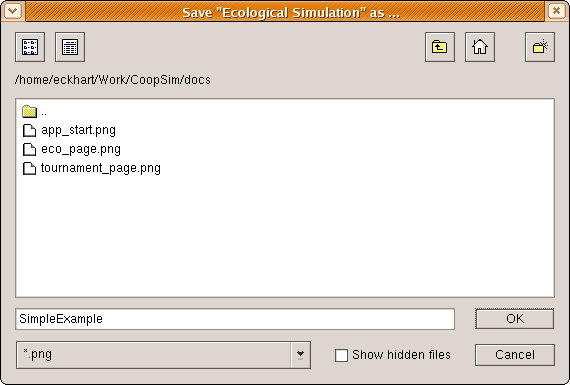
\includegraphics[width=5cm,keepaspectratio]{big_images/save_page_dialog.png}
\end{center}

This does not only work with the \emph{Ecological Simulation} page
but with all other pages as well. So, whenever you want to save some
content you are seeing on the screen, just select \emph{Save Page As}
in the \emph{Edit} menu and you will be prompted to save the content
of the currently selected page. Alternatively, you can select \emph{Copy
Page} in the \emph{Edit} menu (or click the \emph{Copy Page} button
in the toolbar) to copy the content of the selected page to the clipboard.
You can then easily insert the content into another application, say
a word processor, by pressing \emph{Crtl-V} within this application.

Apart from the graph of the ecological simulation, which usually starts with a
uniformly distributed population, you may also want to know how the three
strategies fare in the ecological simulation when they are given different
population shares in the beginning.  For three strategies the population
dynamics can be visualized as a simplex diagram. (If there are more than three
strategies in the simulation then the three strongest strategies are depicted.)
On a simplex diagram each point within the simplex represents a certain
population distribution. The visualization of the population dynamics looks
very similar to a vector field in physics. But, bear in mind that population
dynamics is a discrete process, while vector fields in physics are usually
continuous. (For a more comprehensive explanation of simplex diagrams, look
into the literature on evolutionary game theory, as for example
Maynard-Smith's ``Evolution and the Theory of Games''). If you select the
\emph{Simplex Diagram} page you should see a picture like this:

\begin{center}
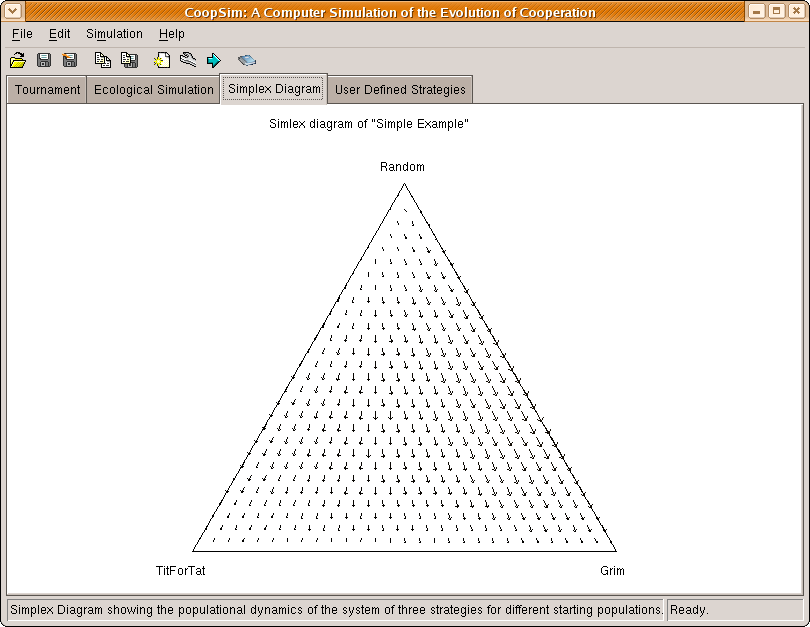
\includegraphics[width=8cm,keepaspectratio]{big_images/simplex_page.png}
\end{center}

The arrows indicate the direction of the ``field'' (i.e. the direction
the population drifts to at a certain point). The length of the arrows
indicates the strength of the drift. Big arrows mean a strong drift
while small arrows indicate an only slow population drift.


\subsection{Defining a new simulation}

Now, you might think, what would happen if we add another strategy to
our tournament? Nothing is easier than that! In order to do so, we have
to create a new simulation setup. This can be done by selecting
\emph{New Simulation} in the
\emph{Simulation} menu or by clicking the \emph{New Simulation} button
in the toolbar (the button before the one with the wrench symbol).
Selecting \emph{New Simulation} opens a dialog where you can define a
new simulation setup based on the current simulation setup. The dialog
looks like this:

\begin{center}
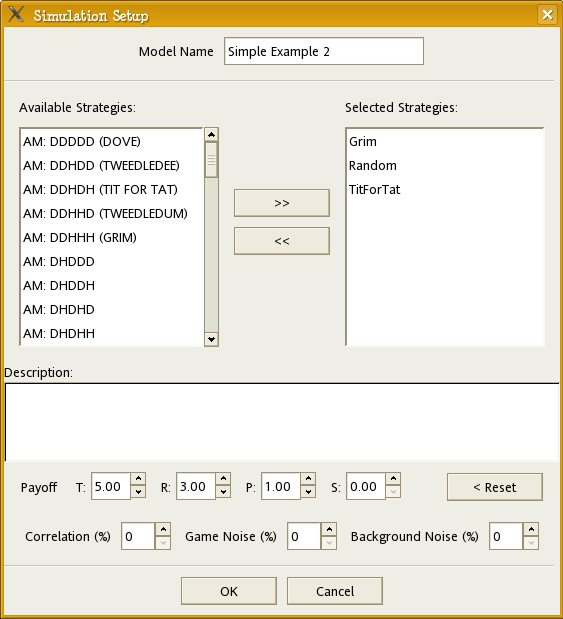
\includegraphics[width=6cm,keepaspectratio]{big_images/new_dialog1.png}
\end{center}

The dialog allows you to select the strategies you want to let take
part in the tournament. You can see the list of available strategies
on the left hand side. On the right hand side you can see the strategies
that will play in the tournament. 

Let us try to add the strategy TESTER to our tournament. In order to
do so, select TESTER with a mouse click in the list box on the left
hand side. (Hint: You may have to scroll the list down a little bit,
before TESTER appears.) Notice that when you select a strategy, an
explanation of the strategy appears in the text box below. When you
have selected TESTER, click on the button ``\emph{>\,>}'' in the middle of
the dialog box. This should transfer TESTER from the list of available
strategies to the list of selected strategies.

\begin{center}
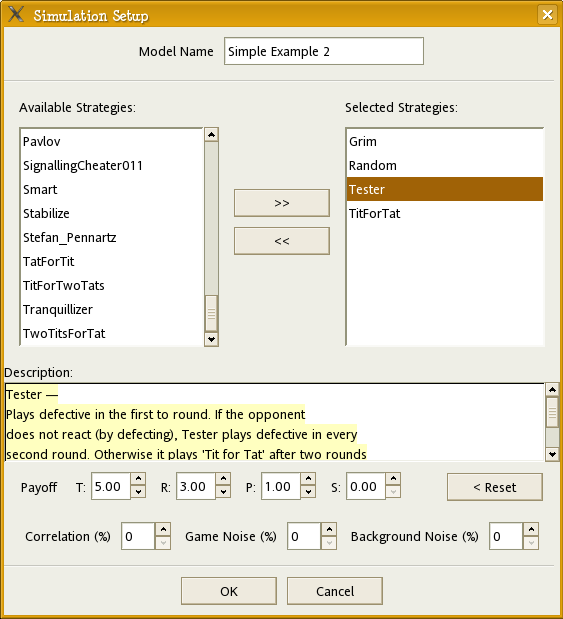
\includegraphics[width=6cm,keepaspectratio]{big_images/new_dialog2.png}
\end{center}

Finally you should enter a name for your new simulation setup in the
text entry widget at the top of the dialog box. Take ``New Example'',
if you do not know what to enter. Now click \emph{O.K.} to see what
happens. Well, since now there are four strategies in the tournament,
there won't be a simplex diagram any more. Select the page \emph{Ecological
Simulation} in order to see what has changed. Obviously, this time
TITFORTAT has come out at the top of the strategies. Although TESTER
has not been very successful itself, it has changed the overall results
dramatically.


\subsection{Programming a new strategy}

The last step of this introductory walkthrough will show you how
to add your own strategies to \emph{CoopSim}, if you know the basics
of the \emph{Python} programming language. For the sake of brevity,
I will only explain how to activate a custom strategy that has already
been coded but deactivated by comment signs. In order to program your
own strategy you have to change to the \emph{User Defined Strategies}
page in the main window. The page contains a simple text editor, where
you can enter python program code:

\begin{center}
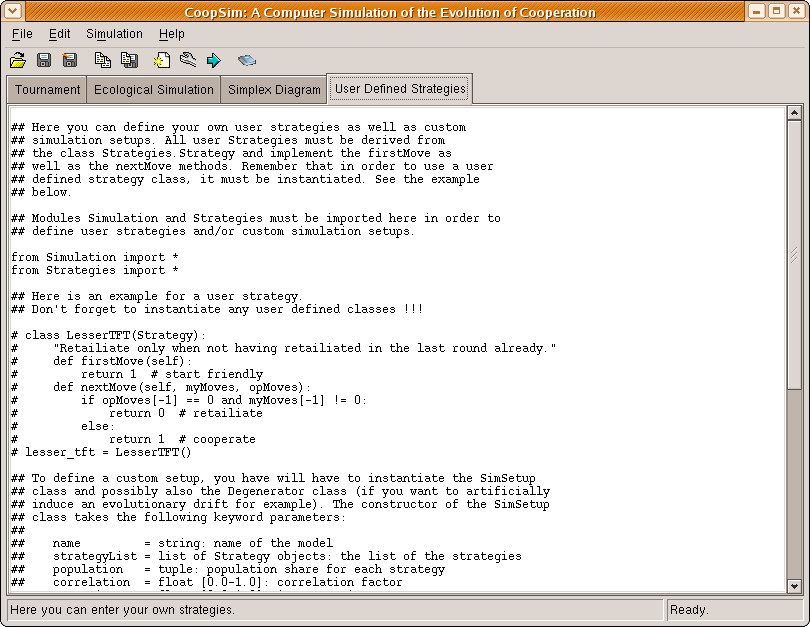
\includegraphics[width=8cm,keepaspectratio]{big_images/user_page.png}
\end{center}

As you can see, there is already quite a bit of program code there.  This
program code has been inserted for explanatory purposes.  Every line starts
with a ``\#'', which is a token for the python interpreter to treat the line
as a comment and not to execute it. Try to locate the class definition of
\emph{class LesserTFT}.  Reactivate this strategy by removing the comment sign
in front of the class definition as well as the following single space
character (this is important) so that the statement ``class
LesserTFT(Strategy):'' starts in the very first column. Do the same for the
following lines up to the line where the class LesserTFT is instantiated. This
is line that reads ``lesser\_tft = LesserTFT()''. Remember that indentation
has syntactical significance in \emph{Python}, so beware of inadvertently
changing the indentation while removing the comment signs and the following
space character.

\begin{center}
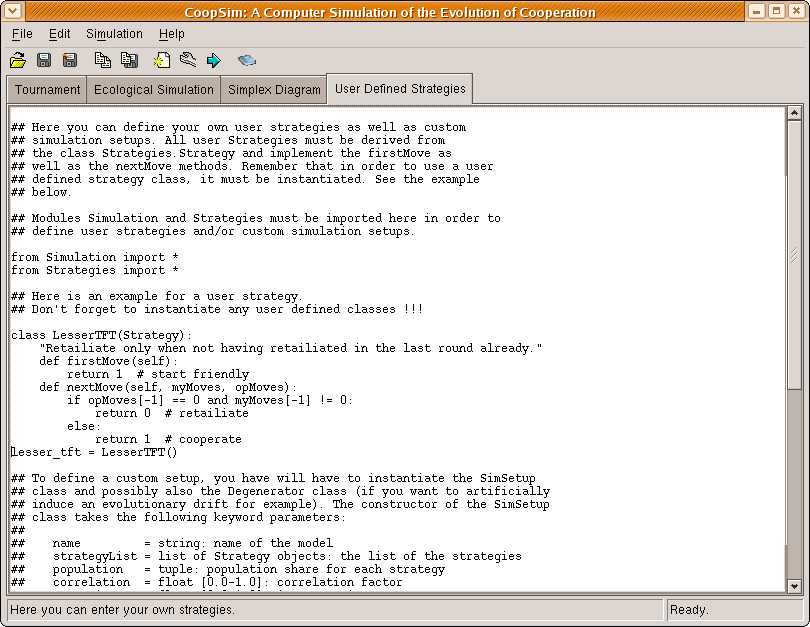
\includegraphics[width=8cm,keepaspectratio]{big_images/user_page_modified.png}
\end{center}

Now select \emph{Edit Simulation} from the \emph{Simulation} menu
(or click on the wrench symbol in the toolbar). If no errors have
occurred in the program code you will now find a new strategy \emph{LesserTFT}
among the available strategies in the simulation setup dialog
box. If you receive an error message, you may have forgotten to delete
a single trailing space after the comment sign ``\#'' in one or
more lines.


\section{Comprehensive Overview}

This Chapter of the manual gives a comprehensive overview over all
menu commands of the \emph{CoopSim} application.


\subsection{File Menu}


\subsubsection{New}

Resets the application to its startup state. This means that all simulation
setups and custom strategies will be deleted. Usually there is not
much need to select \emph{New} at all, except when you get lost.


\subsubsection{Open}

Opens a previously saved state, including all simulation setups as
well as any user defined strategies or setups. All previous simulation
setups will be lost. (There is - at the moment - no way of merging
different simulation setups.)


\subsubsection{Save}

Saves the full application state in a file, including all simulation
setups and and any program code that has been entered in the \emph{User
Defined Strategies} page. 

{\bf Warning:} The save files may not be interchangeable between different
versions (including subversions) of CoopSim! Loading a save file from
a different version of CoopSim may cause CoopSim to crash!

If you want to save program code from the \emph{User Defined Strategies}
page, the best idea is to copy and paste it to a text editor and save
it as a text file.


\subsubsection{Save As}

Promts for a filename and then saves the full application state in
a file, including all simulation setups and and any program code that
has been entered on the \emph{User Defined Strategies} page.

{\bf Warning:} The save files may not be interchangeable between different
versions (including subversions) of CoopSim! Loading a save file from
a different version of CoopSim may cause CoopSim to crash!

If you want to save program code from the \emph{User Defined Strategies}
page, the best idea is to copy and paste it to a text editor and save
it as a text file.


\subsubsection{Exit}

Quits the application.


\subsection{Edit Menu}

As you may have noticed, there is no ``Paste'' entry in the \emph{Edit} menu.
If you want to add some program code from another application, say a python
editor, to your own custom strategies on the \emph{User Defined Strategies}
page, you can access the usual {\em cut}, {\em copy} and {\em paste} functions
on this page via keyboard with \emph{crtl-x}, \emph{crtl-c}, \emph{crtl-v}
respectively.


\subsubsection{Copy Page}

Copies the content of the currently visible page to the clipboard.  This can
either be an image (pages \emph{Ecological Simulation} and \emph{Simplex
  Diagram}) or HTML file (page \emph{Tournament}) or plain ASCII text (page
\emph{User Defined Strategies}).


\subsubsection{Save Page As}

Saves the content of the currently visible page to a file. This can
either be an image (pages \emph{Ecological Simulation} and \emph{Simplex
Diagram}) or plain ASCII text (pages \emph{Tournament} and \emph{User
Defined Strategies}). Currently the only supported file format for
graphical images is the \emph{png} format.


\subsection{Simulation Menu}


\subsubsection{New Simulation}

Invokes the setup dialog for setting up a new simulation. In the setup-dialog
the set of strategies that take part in the tournament can be selected, and
the payoff parameters T (tempation of cheating), R (reward for cooperation), P
(punishment for mutual non cooperation), S (sucker's payoff) and the
parameters \emph{Noise}, \emph{Correlation}, \emph{Background} \emph{noise}
can be adjusted. The latter three of these parameters can be assigned
percentage values from 0 to 100 percent. \emph{Noise} specifies the in game
noise that is a random probability with which the move of a player is turned
into its opposite.  \emph{Correlation} determines how often players meet with
players of their own kind. It ranges from totally random (= 0 \%) to the
closest possible correlation when only players of the same type meet (= 100
\%).  (Try a tournament between DOVE and HAWK and change this parameter in
steps of 10 \% from 0 \% to 50 \%. What can you observe?)  \emph{Background
  noise} specifies an evolutionary background noise meaning that reproduction
does depend on the fitness plus/minus a certain random factor.

\subsubsection{Edit Simulation}

Same as \emph{New Simulation}, only that the current simulation setup
is manipulated instead of creating a new simulation setup. Simulation
setups that have been programmed on the \emph{User Defined Strategies}
page can not be edited. You will have to create a new simulation setup
instead. In this case the parameters \emph{population} and
\emph{mutators} will be reset to their default values in order to
avoid incongruous setup data. (Setup data would become incongruous if
it specifies the mutation of a strategy to another strategy that
has manually been removed from the setup).


\subsubsection{The \emph{Simulation Setups}}

Following in the \emph{Edit} menu is a list of simulation setups.
Whenever you define a new simulation setup it appears in this list.
The currently selected simulation setup is marked. You can run or
restart a simulation by selecting it from this menu.


\subsubsection{Remove Models}

Opens a dialog that allows you to remove setups that you do not need
any more from the \emph{Simulation} menu.


\subsection{Help Menu}

\subsubsection{Help}

Shows this manual as HTML text in a browser window.

\subsubsection{License}

Shows the license agreement for this software. This software is open
source under the GNU Public License.

\subsubsection{About}

Tells you who wrote this program.


\section{Advanced Topics}

\subsection{Technical notes on the dynamical model}

Population dynamics crucially depends on two factors: How fitness
is transformed into a reproduction rate (assuming that the transformation
is always monotonous, this still leaves open quite a number of possibilities),
and whether or when species die out. The model used in \emph{CoopSim}
uses population shares rather than an integer number of individuals
for each species (strategy). This means that species never die out,
even though their population share might become arbitrarily small.
The reproduction rate is determined by the score a strategy gains
in the tournament divided by the average score. Thus the reproduction
rate does depend on the payoff parameters. Both assumptions
are to a certain degree arbitrary.

Evolutionary noise (which can be adjusted via the \emph{Background
noise} parameter in the simulation setup dialog) is modeled as random
disturbance on the reproduction rate (not on the population share).



\subsection{Programming user strategies}


\subsubsection{Preface}

There are two ways of adding user strategies to \emph{CoopSim}: Either by
entering them on the \emph{User Defined Strategies} page when the application
is running or by writing them directly to the \emph{Strategies.py} module of
the program code. Since \emph{CoopSim} is open source software and thus comes
with the complete source code you can easily do so. Except for experimenting,
the latter method of adding your own strategies directly to the program code
is probably the better one, because entering strategies on the \emph{User
Defined Strategies} page is more error prone and can quickly get frustrating.
Also, changing the module \emph{Strategies.py} can be done with a real python
editor with syntax highlighting, class browser and other comforts. On the
other hand, you should only change \emph{Strategies.py} if you really know
what you are doing, or otherwise \emph{CoopSim} might not run any more.


\subsubsection{The \emph{Strategy} class}

Any strategy in the game must be derived from \emph{class Strategies.Strategy}.
This class defines the two methods \textbf{firstMove}(self) and
\textbf{nextMove}(self, myMoves, opMoves). Both methods must return
either 0 or 1, where 0 means ``defection'' and 1 stands for
``cooperation''. \emph{firstMove} does not take any parameters except
``self'', while \emph{nextMove} gets the list of its own moves
during the previous rounds of the current match as well as a list
of its opponents previous moves. Both lists are list of zeros and
ones. Implementing your own user strategies is pretty easy now: Simply
derive a class from \emph{class Strategies.Strategy} and define the
methods \emph{firstMove} and \emph{nextMove}, nothing else is needed,
neither a constructor, nor is it necessary to worry about a name for
the strategy, because the class name is automatically used as the
strategies' name. All state saving variables of your class 
must be reset in  method {\em firstmove}! This is necessary, because
the same strategy object is used in all matches of the tournament.
Here is a simple example of a custom strategy class:

\begin{verbatim}
class LesserTFT(Strategy):    
    """Retailiate only when not having retailiated in    
    the last round already.    
    """
    def firstMove(self):
        return 1  # start friendly
    def nextMove(self, myMoves, opMoves):
        if opMoves[-1] == 0 and myMoves[-1] != 0:
            return 0  # retailiate
        else: 
            return 1  # cooperate

# Do not forget to instantiate your class, otherwise
# it will not appear among the available strategies!

lesser_tft = LesserTFT()
\end{verbatim}


\subsection{Defining user setups}

There are many more parameters that determine a simulation than can be
edited through the simulation setup dialog. To change these
parameters, thereby gaining access to a much wider range of possible
simulation scenarios, it is necessary to define the simulation setup
manually on the {\em User Defined Strategies} page. 

All parameters that determine a simulation's behaviour are defined in
an object of \emph{class Simulation.SimSetup}. To define a simulation
setup, it suffices to instantiate this class with the needed
parameters. Here is an explanation of the parameters the constructor
of the SimSetup class takes:

\begin{verbatim}

    name         = string: name of the model
    strategyList = list of Strategy objects: the list of the strategies
    population   = tuple: population share for each strategy
    correlation  = float [0.0-1.0]: correlation factor
    gameNoise    = float [0.0-1.0]: in game noise
    noise        = float [0.0-1.0]: evolutionary background noise
    iterations   = int:  number of iterations for one match
    samples      = int:  number of sample matches to take (only useful for 
                   randomizing strategies)
    payoff       = tuple of floats:  payoff tuple (T, R, P, S)
    demes        = DemeDescriptor: defines the deme structure of the
                   population or `None' if there is only one deme
    mutators     = list of Mutator objects: description of possible
                    mutation (or degeneration resp.) of strategies during 
		    the course of the evolutionary development.
    cachedPM     = cached payoff matrix
    cachedLog    = cached tournament log string

\end{verbatim}

The most interesting use for programmed setups is setups with
\emph{mutators}. Mutators describe a genetic drift of certain strategies 
into another type of strategy. For
example one could imagine a certain percentage of TITFORTAT players
degenerating into DOVE every generation, because they weren't really
able to understand the principle of TITFORTAT. The assumption of
degeneration has great consequences for the topics of evolutionary
stability and the like. Here is an example of a simulation setup
with a non uniform population consisting of the strategies GRIM, DOVE
and TESTER, where GRIM degenerates to DOVE at a rate of one percent per
generation. (Try this one out and let the ecological simulation
continue for at least 400 generations. What can you observe?)

\begin{verbatim}
custom_setup = SimSetup(name         = "Grim => Dove, Tester",
                        strategyList = [Grim(), Dove(), Tester()],     
                        population   = (0.8, 0.01, 0.19), 
                        mutators     = [Mutator(0,1,0.01)])
\end{verbatim}


\section{Further Reading}

For those who would like to learn more about the game theoretical
foundation of {\em CoopSim}, here are a few good books on this
topic:

\setlength{\parindent}{0ex}
\setlength{\parskip}{2ex}

{\bf Axelrod, Robert (1984)}: Die Evolution der Kooperation,
Oldenbourg, Mnchen (5 Aufl. 2000; engl. Original 1984).

{\bf Axelrod, Robert (1997)}: The Complexity of Cooperation. Agent-Based Models of
Competition and Collaboration, Princeton University Press, Princeton.

{\bf Binmore, Ken / Samuelson, Larry (1992)}: Evolutionary Stability in
Repeated Games Played by finite Automata, in: Journal of Economic Theory 57
(2/1992), 278-305.

{\bf Binmore, Ken (1994)}: Game Theory and the Social Contract I. Playing
Fair, MIT Press, Cambridge (Massachusetts), London (England) (4. Nachdruck
2000).

{\bf Binmore, Ken (1998)}: Game Theory and the Social Contract II. Just
Playing, MIT Press, Cambridge (Massachusetts), London (England).

{\bf Maynard Smith, John (1982)}: Evolution and the Theory of Games, Cambridge
Univ. Press, Cambridge (8. Aufl. 2000).

{\bf Schuessler, Rudolf (1990)}: Kooperation unter Egoisten: vier Dilemmata,
R.Oldenbourg Verlag, Muenchen (2.Aufl. 1997)

After having occupied myself with computer simulations of this type for a
longer time, my own opinion about the scientific value and particularly the
explanatory power of this brand of simulations has become very critical.  If
curious, you may want to read some of my papers on this topic:

\href{http://www.eckhartarnold.de/papers/2015_How_Models_Fail/How_models_fail.html}{How
  Models Fail. A Critical Look at the History of Computer Simulations
  of the Evolution of Cooperation, in: Philosophical Studies (forthcoming 2015)}

\href{http://www.eckhartarnold.de/papers/2014_Social_Simulations/Whats_wrong_with_social_simulations.html}{What's
  wrong with social simulations?, in: The Monist 2014 (97,3), 361-379, DOI: 10.5840/monist201497323}

\href{http://www.eckhartarnold.de/papers/2013_Simulations_as_Logical_Possibilities/Arnold_2013_Simulations_as_Proofs_of_Logical_Possibilities.pdf}{Simulation  Models  of   the  Evolution  of   Cooperation  as Proofs of  Logical Possibilities. How Useful Are They?, in: Etica \& Politica
/ Ethics \& Politics, XV, 2013, 2, pp. 101-138}

\end{document}
